

\documentclass{article} 

\usepackage{amsmath} % \usepackage is a command that allows you to add functionality to your LaTeX code
\usepackage{graphicx}
\usepackage{hyperref}

\graphicspath{ {./plots} }

\title{Raport for Flight Delay Predicion Project} % Sets article title
\author{Dominik Olejarz, Patryk Rybak, Maksymilian Wnuk} % Sets authors name
\date{\today} % Sets date for date compiled

% The preamble ends with the command \begin{document}
\begin{document} % All begin commands must be paired with an end command somewhere
 \maketitle
    
 \section{Problem Statement} % creates a section

Our goal is to predict flight delays and, in the future, expand the program to calculate the most probable delay values. Throughout our work, we will utilize a dataset containing flight information from 2017 to 2018, provided by the Bureau of Transportation Statistics in conjunction with the Weather API. The primary focus is to examine the correlation between weather conditions and flight delays.

Our approach centers around machine learning techniques, and we will employ statistical learning models using Python. The aim is to forecast flight delays and in future provide precise values of delays. We believe that our project can contribute to improving the travel experience by offering more accurate information about potential flight delays.

    
 \section{Data downloading}
Getting data for our machine learning models requires two combined datasets, 
flights and weather:
	\subsection{Flights data}
		We are getting 2017-2018 flights data from \url{kaggle.com} website.
		It contains of columns:	
			\begin{itemize}
\item Airline 
\item Origin city 
\item Destnation city
\item Arr time  
\item Cancelled 
\item Delay  
\item Distance  
				
			\end{itemize}

	\subsection{Weather data}
		Fetching data for weather requires more work than just downloading a csv file.
		We will be downloading it by making api requests to \url{https://www.visualcrossing.com}.
		Thanks to Visual Crossing\textsuperscript{\tiny\textregistered} company, we were able to make those requests in unlimited way.
		We contacted their support and then they gave us access to unlimited api key. We
		get columns:

			\begin{itemize}
\item Temperature
\item Cloudcover
\item Monphase
\item Windspeed, windgust and winddir
\item Snow and snowdepth
\item Dew humidity
\item Ice and freezing rain
				
			\end{itemize}


\section{Merging data}

DOMINIK

\section{Plots}
In this section we will look at plots describing data in our dataset.
	
	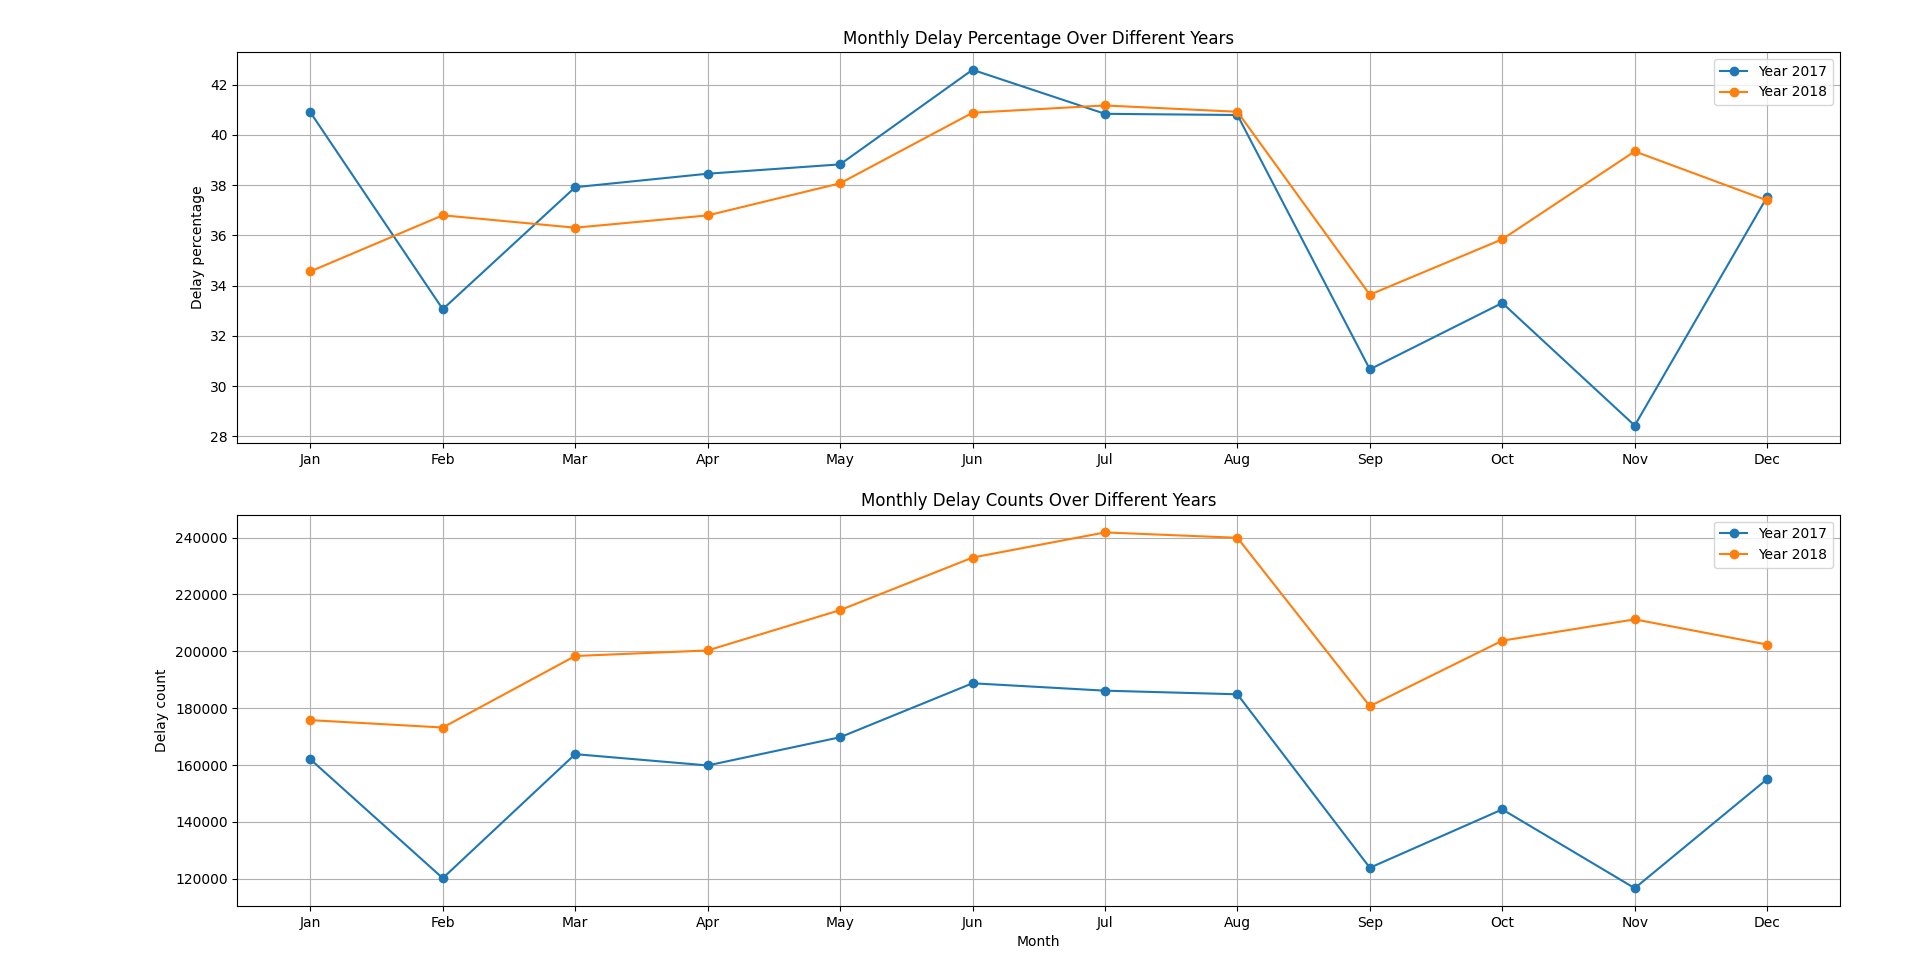
\includegraphics[scale=0.22]{plot1}
	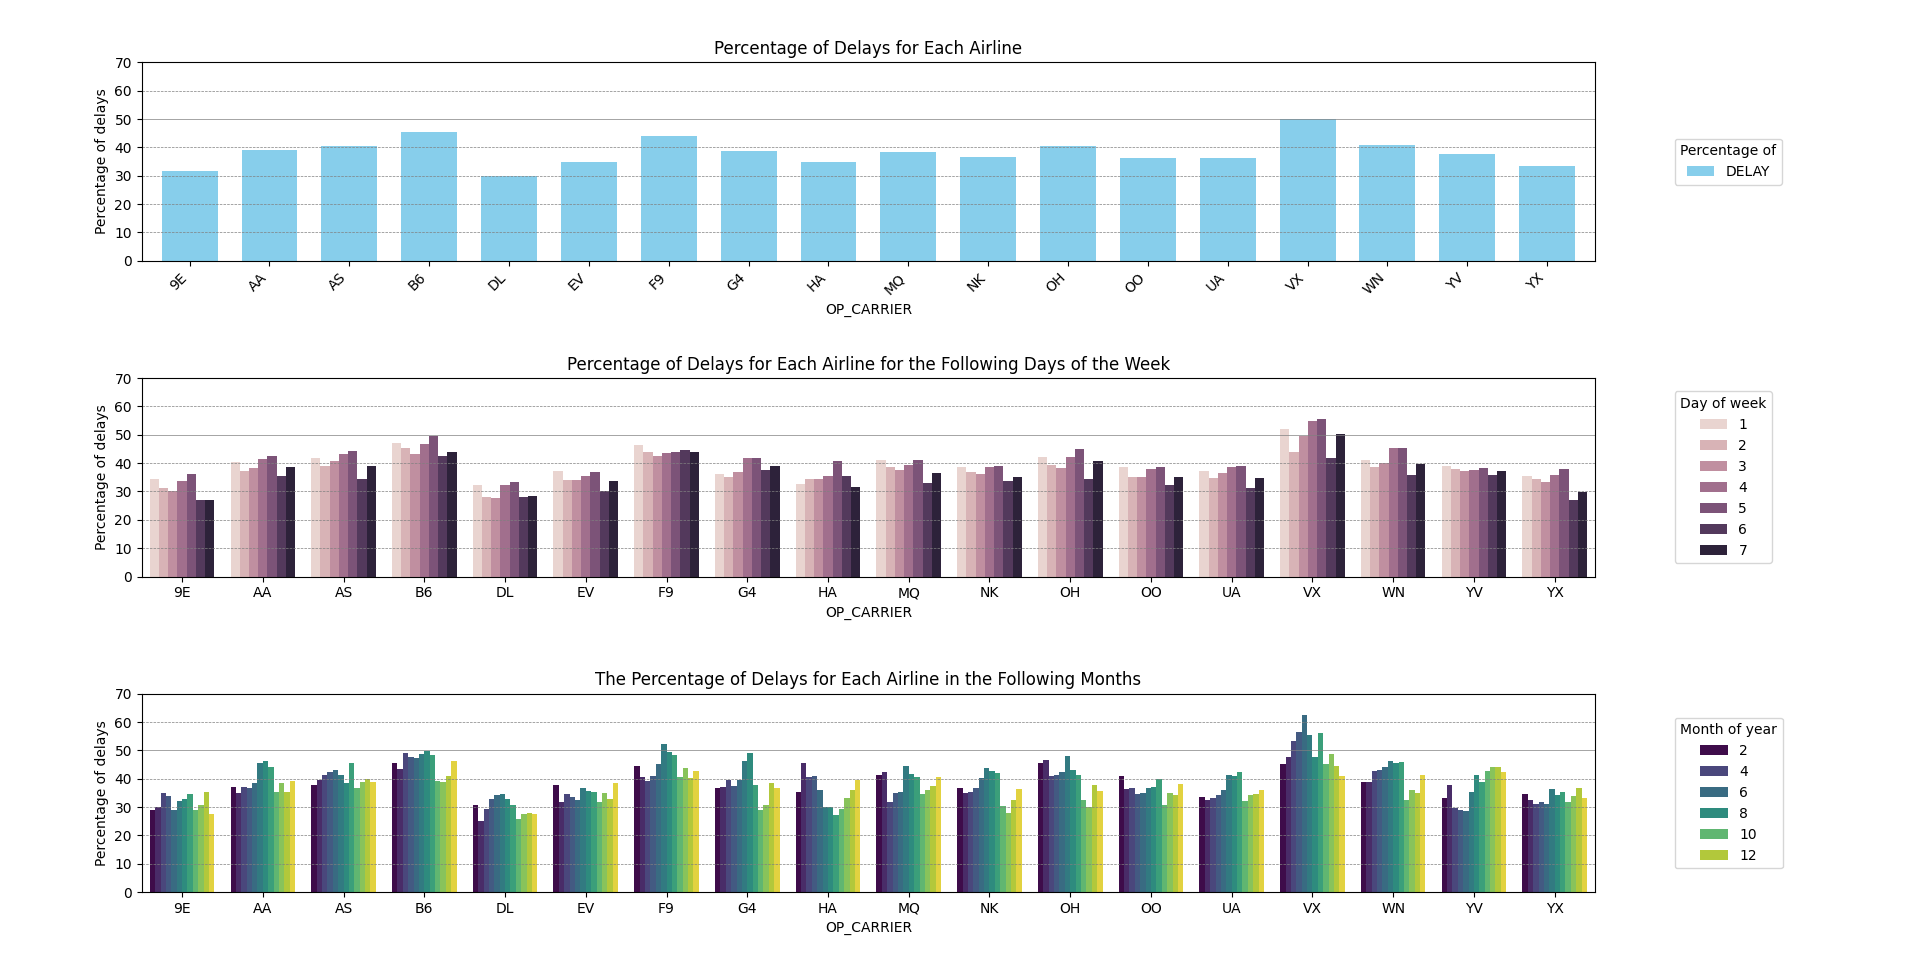
\includegraphics[scale=0.25]{plot2}
	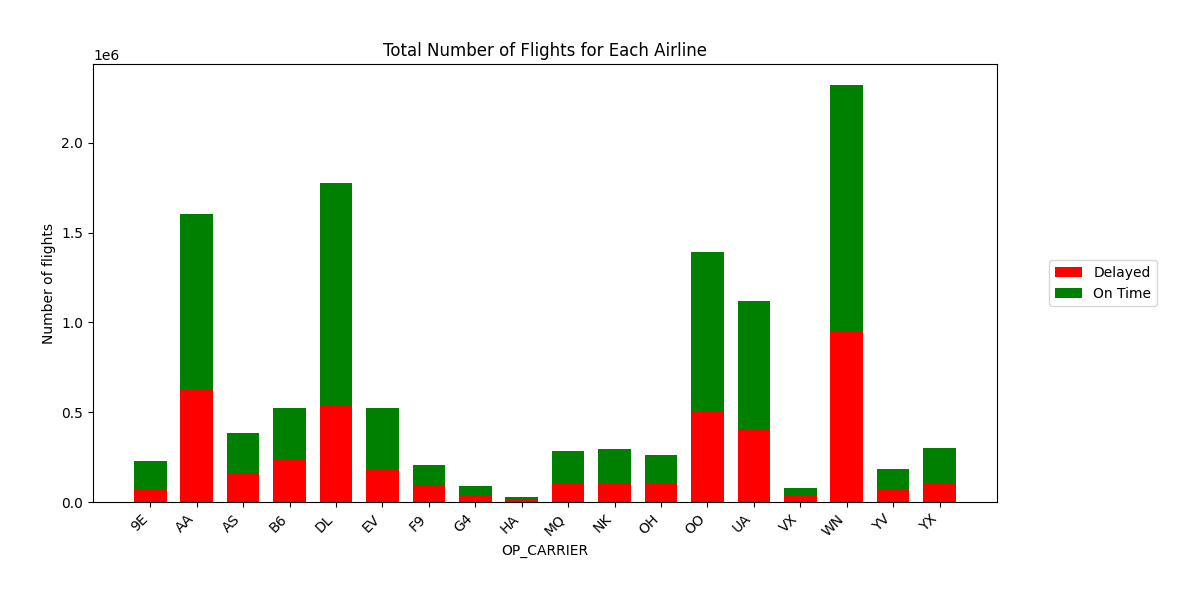
\includegraphics[scale=0.4]{plot3}
	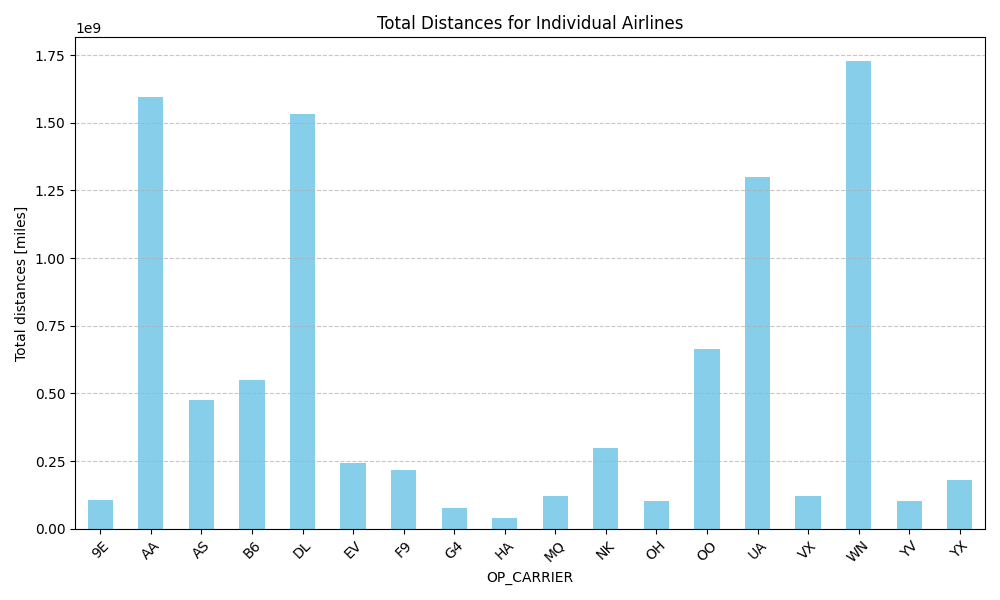
\includegraphics[scale=0.4]{plot4}	


\section{Data preprocessing}
Dataset contains of lots of NaN's. We removed all of them, by removing rows that contained them. Data loss
was incredibly low, we lost about 10,000 of rows that contained at least one NaN, which is great. Additionally,
we removed columns that contained A LOT of NaN's. Those columns were:
	\begin{itemize}
		\item Windgust -75.22\% NaNs
		\item Snow - 8.13\% NaNs
		\item Snowdepth - 8.13\% NaNs
		\item ID,id - 55\% and 44\% respectively,no idea why so many nans, its just id's whose we don't even use in our model.
	\end{itemize}


However, we are not sure if that was proper way of doing this, hence we ask ourselves: does snow affect flight delays? How about snowdepth and wingust? Later on we can always retrieve those columns and check correlation.

\section{Machine learning part}

\end{document} % This is the end of the document
